\begin{problem}{Forgotten Land}{standard input}{standard output}{3 seconds}{512 megabytes}

Fytelandian scientists are famous for their love for historical research. Recently they have discovered the remains of $n$ cities, which definitely belonged to a great past civilization.

All the discovered cities were connected by exactly $n-1$ roads, and there was exactly one way to move between any pair of cities using these roads. The scientists found a lot of writings in each city and concluded that people of the civilization spoke $k$ different languages. In city $v$ people spoke language $a_v$.

It is known that the cities formed several alliances, and each city belonged to exactly one alliance. However, the exact formation of alliances remains unknown.

Let's say that an alliance is an arbitrary set of cities $c_1, c_2, \ldots, c_m$ that might or might not be connected by roads. To rule the alliance it was necessary to be able to make connections between different cities with people who speak different languages. The head of the alliance had to support all languages that were spoken either in some city $c_i$ of the alliance or in some city on the shortest path between some two cities $c_i$ and $c_j$ of the alliance.

The more languages were supported in the alliance, the harder was the translator's job~--- a good translator had to speak all of them! Luckily, many languages were similar to each other, and the more languages the translator had known, the easier it was for them to learn a new language. Every consecutive new language took twice less time for the translator to learn. 

Let's say that the \textit{language difficulty} of the alliance is the time the translator needed to spend to learn all languages supported in the alliance. The first language took $2^k$ units of time to learn, thus, the language difficulty of the alliance is equal to $2^k+2^{k-1}+\ldots+2^{k+1-t}$, where $t$ is the number of different languages supported in the alliance. Note that as there are $k$ languages in total, this sum is always an integer.

Let's say that an \textit{alliance partition} is a partition of all cities into several alliances. Two alliance partitions are considered different if there exist two cities $u$ and $v$ such that they belong to the same alliance in one partition and to different alliances in the other partition.

Let's say that the \textit{plausibility} of an alliance partition is the sum of the language difficulties of all alliances in the partition.

You need to calculate the sum of the plausibilities of all possible alliance partitions. As this number can be very big, you need to find only its remainder modulo $998\,244\,353$.


\InputFile
The first line of the input contains two integers $n$ and $k$~--- the number of cities and the number of languages, respectively ($1 \le n \le 5000$; $1 \le k \le 10$).

The second line contains $n$ integers $a_1, a_2, \ldots, a_n$~--- the languages spoken in the cities ($1 \le a_i \le k$).

Each of the following $n - 1$ lines contains two integers $u_i$ and $v_i$~--- cities connected by the $i$-th road ($1 \le u_i, v_i \le n$).

\OutputFile
Output the sum of the plausibilities of all possible alliance partitions modulo $998\,244\,353$.

\Examples


\exmpthreewidinf=0.25\thelinewidth
\exmpthreewidouf=0.25\thelinewidth
\exmpthreewidnote=0.40\thelinewidth
\def\kwExampleNotes{Illustration}

\begin{examplethree}
\exmp{3 2
1 2 1
1 2
2 3
}{48
}{
\vspace{1mm}
\center
\includegraphics[scale=0.5]{001.eps}
}%
\exmp{6 4
1 2 1 3 4 2
1 2
2 3
3 5
3 4
2 6
}{14504
}{
\vspace{1mm}
\center
\includegraphics[scale=0.5]{002.eps}
}%
\end{examplethree}

\Note
In the first example, there are three cities. Consider all possible alliance partitions:

\begin{itemize}
\item {
 Three alliances:
 \begin{itemize}
  \item \{1\}. One city, the only supported language is language 1. The language difficulty is $2^2=4$.
  \item \{2\}. One city, the only supported language is language 2. The language difficulty is $2^2=4$.
  \item \{3\}. One city, the only supported language is language 1. The language difficulty is $2^2=4$.
 \end{itemize}
 The plausibility of this partition is $4+4+4=12$.
}
\item {
 Two alliances:
 \begin{itemize}
  \item \{1, 2\}. Two cities, languages 1 and 2 are supported. The language difficulty is $2^2+2^1=6$.
  \item \{3\}. One city, the only supported language is language 1. The language difficulty is $2^2=4$.
 \end{itemize}
 The plausibility of this partition is $6+4=10$.
}
\item {
 Two alliances:
 \begin{itemize}
  \item \{1, 3\}. Two cities, languages 1 and 2 are supported. Note that even though the only language spoken in the alliance is language 1, language 2 is supported as well because it's spoken in city~2 that lies on the shortest path between cities 1 and 3. The language difficulty is $2^2+2^1=6$.
  \item \{2\}. One city, the only supported language is language 2. The language difficulty is $2^2=4$.
 \end{itemize}
 The plausibility of this partition is $6+4=10$.
}
\item {
 Two alliances:
 \begin{itemize}
  \item \{1\}. One city, the only supported language is language 1. The language difficulty is $2^2=4$.
  \item \{2, 3\}. Two cities, languages 1 and 2 are supported. The language difficulty is $2^2+2^1=6$.
 \end{itemize}
 The plausibility of this partition is $4+6=10$.
}
\item {
 One alliance:
 \begin{itemize}
  \item \{1, 2, 3\}. Three cities, languages 1 and 2 are supported. The language difficulty is $2^2+2^1=6$.
 \end{itemize}
 The plausibility of this partition is $6$.
}
\end{itemize}

The required sum is equal to $12+10+10+10+6=48$.

\end{problem}

